\chapter{Lenguaje de Actor Mínimo}

En esta sección se explorará la sintaxis de un lenguaje que implementa los rudimentos que vimos en la sección anterior, tales como comportamientos, creación de nuevos actores, creacion de nuevas comunicaciones, etc. El lenguaje \SAL fue desarrollado con inteciones pedagógicas y tiene una sintaxis parecida a la de Algol. 

Se utilizará la notación \textbf{Backus-Naur} para definir la sintaxis, se utilizá \textbf{*} para denotar una o más ocurrencias del termino. Muchas veces se suele codificar en las gramáticas la presedencía de operadores, no se sigue este patron.

\section{Expresiones}
Existen tres tipos primitivos, booleanos, enteros y dirección del buzón. Las operaciones
posibles entre los booleanos son \textbf{or}, \textbf{and}, \textbf{not}. Con
respecto a los enteros se pueden operar utilizando \textbf{+}, \textbf{-},
\textbf{*}, \textbf{/}.
La dirección de un buzón es un identificador que es devuelto cuando se crea un nuevo actor, 
este tipo de primitivo no tiene nigún operador asociado.

La gramática de las expresiones booleanas es la siguiente:

\begin{grammar}
<exp> ::= <term> `or' <term> | <term> `and' <term> 
  
<term> ::= <bool> | `not' <term> | `(' <exp> `)' 

<bool> ::= `TRUE' | `FALSE'
\end{grammar}

La gramática de los enteros es la siguiente:

\begin{grammar}
<exp> ::= <term> `*' <term> | <term> `/' <term>  
  \alt <term> `+' <term>  | <term> `-' <term>

<term> ::= <numero> "*" | `-' <term> | `(' <exp> `)'

<numero> ::= `1' | `2' | `3' | `4' | `5' | `6' | `7' | `8' | `9' | `0'
\end{grammar}


\section{Definición de comandos}
La gramática de los comandos en SAL es la siguiente:

\begin{grammar}
  <command> ::= `send' $e_1, e_2, \ldots\ , e_n$ `to' <actor>  
  \alt `become' $B(e_1, e_2, ..., e_n)$
  \alt `let' $x_1$ = `new' $B_1(e_1, e_2, ..., e_{1n})$, \\
   \ldots\ \ $x_k$ = `new' $B_k(e_1, e_2, ..., e_{kn})$   \\
  `in' <command> 
  \alt `if`<bool-expr> `then' <command> `else' <command> `end if'
  \alt <command> `||' <command>
\end{grammar}

\begin{description}
\item [send] Este comando permite enviar mensajes a otros actores, toma como
  parámetro una lista separada por coma de las expresiones a enviar, y el actor
  destino, el envío de mensajes es asincrónico. Cada expresión es evaluada antes
  de ser enviada.
\item [become] Este comando especifica el siguiente comportamiento del actor
  que está procesando la comunicación recibida. Como en el caso anterior se evalúan
  las expresiones antes de ser enviadas, y estas aparecerán como la listas de
  parámetros del comportamiento. 
\item[new] Este comando sirve para crear nuevos actores. El alcance de los
  identificadores de los nuevos actores creados está sujeto al cuerpo de \textbf{let}.
\item[condicional] Luego de evaluar la expresión booleana, si es verdadera
  ejecuta lo que esta a continuación de \textbf{then}, en caso contrario lo que está a
  continuación de \textbf{else}. Funciona como cualquier condicional.
\item[composición] Estos dos comandos en \SAL son ejecutados concurrentemente.
 
\end{description}

La ejecución de los comandos ocurre cuando el actor recibe un mensaje, y todos
ellos ocurren concurrentemente, la composición no es secuencial.

\section{Definición de comportamientos}

La sintaxis de los comportamientos es la siguiente:

\begin{grammar}
<BDef> :== `def' <beh name> `(' <acquaiantence-list> `)' `[`'<input-list>`]' \\
\quad \quad <command>*  \\
\quad `end def'
  
<acquaiantence-list> :== <id> | <id>`,' <acquaiantence-list>
  
<input-list> :== <id> | <id>`,' <input-list>
\end{grammar}

El identificador \textit{beh name} esta atado a una abstracción y tiene alcance
a todo el programa. Los identificadores \textit{acquaiantence-list} los recibe el
momento de instanciación y tiene alcance en todo \textit{command}. Los
identificadores \textit{input-list} son completados al momento de procesar una comunicación
mensaje, y su alcance es todo \textit{command}. 
Ambas listas, \textit{input-list} y \textit{acquaiantence-list} contienen todos
los identificadores libres que están en \textit{command}. Existe un
identificador especial \textit{self} que puede ser utilizado para hacer
referencia al actor que está se definiendo. 
La ejecución de \textit{command} deberá contar a lo sumo con un solo comando
\textit{become}, esta propiedad tiene que ser garantizado de manera estática, de no
existir ningún comando \textit{become}, el actor asumirá un comportamiento de
tipo \textit{bottom}, es es básicamente ignorar los mensajes que se le envíen.


\section{Ejemplos}

En esta sección mostraremos dos ejemplos de \SAL y alguas particularidades del lenguaje. 
Primero se presentará el ejemplo de código, a continuación una breve descripción linea por linea de la funcionalidad, 
y para terminar notas sobre su funcionamiento.

\subsection{Cálculo del factorial}

Está implementación del factorial está adaptada de \cite{Agha:1986:AMC:7929}, esta
depende de un actor \textit{main} que le envía el valor a calcular. El factorial
esta siempre disponible para procesar la siguiente comunicación, no bloquea con
el calculo recursivo del factorial sino que lo delega en otros actores.

La palabra reservada \textit{self} hace referencia a la dirección de buzón
correspondiente al actor que está procesando la comunicación, este es inicializado
cuando el actor es creado.

\begin{lstlisting}[language=sal, style=simple]
def Factorial()[val, customer]
  become Factorial() ||
  if val = 0 then
  send [1] to customer
  else
    let cont = new FactorialCont(val, customer)
       in send [val - 1, cont] to self
  end if 
end def

def FactorialCont(n, customer)[m] 
  send [n * m] to customer
end def

def Main() 
  let fact = new Factorial() 
    in send [3, self] to fact
end
\end{lstlisting}

\begin{description}

\item [Linea 1] $Factorial$ no recive ningún parametro en el momento de ser inicializado, pero si recibe dos parametros cuando procesa una comunicación, la tupla $[val, customer]$ un entero y una la dirección de un buzón respectivamente.
\item [Linea 2] Asigna como siguiente comportamiento a $Factorial()$, sin parámetros ya que $Factorial$ no recibe ningún parametro a la inicialización. El operador $||$ es la composición de SAL, es similar a el $;$ en $C$. 
\item [Linea 3] Envía una tupla con el valor $1$ al actor con buzón $customer$.
\item [Linea 6] Crea un actor de tipo $FactorialCont$. En este caso se utiliza $new$, ya que se está creando un nuevo buzón, y este se asigna a la variable $cont$. Cuando se asigna el nuevo comportamiento, este recive los parametros $val$ y $customer$.
\item [Linea 7] Envia un mensaje a la dirección del buzón propio utilizando la palabra reservada $self$, con la tupla $val - 1$ y la dirección del buzón que se acaba de crear.
\item [Linea 11] $FactorialCont$ recive dos valores cuando es instanciado: un entero $n$ y la dirección de un buzón $customer$. Cuando procesa un mensaje, en su \textit{acquaiantence-list} recive un entero $m$.
\item [Linea 12] Envía la mutiplicación $n*m$ como tupla a la dirección del buzón $customer$ 
\item [Lineas 15-18] Inicializa el actor $Factorial$ y le envia a este la tupla con los valores $3$ y la dirección del buzón actual. 

\end{description}

Concretamente, el actor ante un entero distinto de cero ejecuta dos acciones, crea un actor con
un comportamiento que será multiplicar por \textbf{n} el valor recibido y
enviarlo al buzón de quien pidió el calculo del factorial de \textbf{n}.
También, se envía un mensaje a si mismo para evaluar el factorial de \textbf{n - 1}, y como dirección de cliente utiliza la dirección del buzón del actor
recientemente creado. 

Esto establece una red de actores que multiplicaran por  el valor indicado enviaran el cálculo al siguiente actor en la red, y el último actor 
en la red se lo enviará a quien originalmente lo pidió. 

En la figura \ref{fig:factorial} se puede ver que el actor $Factorial()$ recive como comunicación la tupla $[3,c]$, esto hace que se cree un actor nuevo $c1$, que recibe dos parametros en la inicialización el valor $3$ y la dirección de buzón inicial que recibió como comuncación $Factorial()$, al mismo tiempo auto envía la comuncación con la tupla $[2,c1]$ que es el entero recibido decremetnado en uno y la dirección del buzón del actor creado. Esta ultima tupla inicia el mismo proceso antes descripto, es decir, crea un nuevo actor el cual se inicializa con la dirección de buzón recibida en la comunicación y el entero que recibió decrementado en uno. Todo esto continua hasta que el primer valor de la tupla recibido por $Factorial()$ es cero. 

Cuando el primer elemento de tupla recibido como comunicación es cero, esto hace que se le envie al actor cuya dirección de buzón fue recien recibida la tupla con el valor uno. Este será el ultimo actor creado, que le enviará al siguiente actor el valor de la multiplicación $1*1$, este último le enviará al siguiente actor la multiplicación del valor recibido $2*1$, y el último actor en esta cadena el enviará el resultado de multiplicar $2*3$ al actor $c$, quien fue el que originalmente inició esta cadena.

\begin{figure}[H]
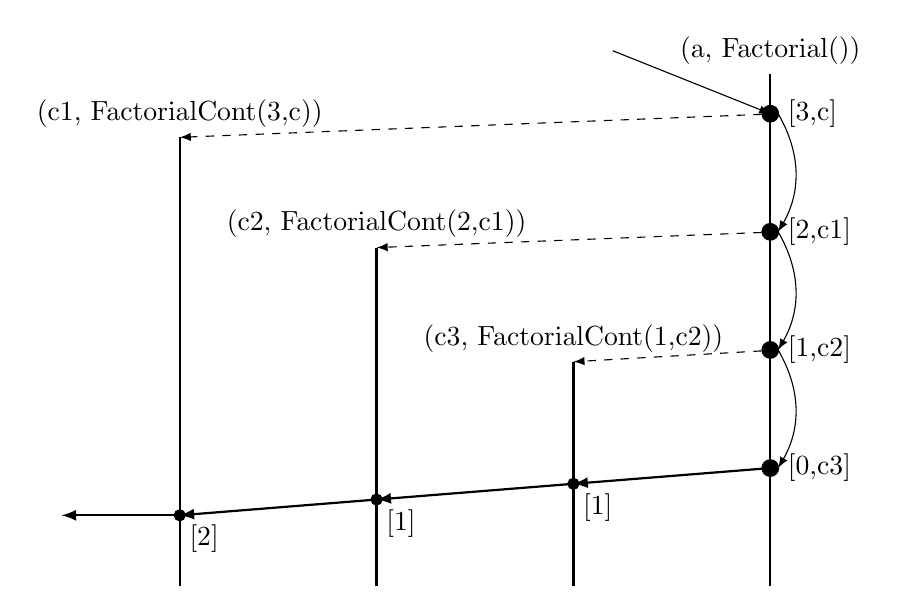
\begin{tikzpicture}

\draw[-latex] (6,7.3) to (8,6.5);

\draw[thick] (8,7) -- (8, 0.5);

\node[] (a1) at (8,7.3) {(a, Factorial())};

\node[align=center, right] (a1) at (8.1,6.5) {[3,c]};
\draw[fill] (8,6.5) circle (3pt);

\node[align=center, right] (a2) at (8.1,5) {[2,c1]};
\draw[fill] (8,5) circle (3pt);

\node[align=center, right] (a3) at (8.1,3.5) {[1,c2]};
\draw[fill] (8,3.5) circle (3pt);

\node[align=center, right] (a4) at (8.1,2) {[0,c3]};
\draw[fill] (8,2) circle (3pt);

\draw[-latex] (a1.west) to[bend left] (a2.west);
\draw[-latex] (a2.west) to[bend left] (a3.west);
\draw[-latex] (a3.west) to[bend left] (a4.west);

\node[] (d1) at (0.5,6.5) {(c1, FactorialCont(3,c))};
\draw[thick] (d1.south) -- (0.5, 0.5);

\node[] (c1) at (3,5.1) {(c2, FactorialCont(2,c1))};
\draw[thick] (c1.south) -- (3, 0.5);

\node[] (b1) at (5.5,3.65) {(c3, FactorialCont(1,c2))};
\draw[thick] (b1.south) -- (5.5, 0.5);

\draw[fill] (5.5,1.8) circle (2pt);
\node[align=center, right] (b2) at (5.5,1.5) {[1]};

\draw[fill] (3,1.6) circle (2pt);
\node[align=center, right] (c2) at (3,1.3) {[1]};

\draw[fill] (0.5,1.4) circle (2pt);
\node[align=center, right] (d2) at (0.5,1.1) {[2]};

\draw[-latex, thick] (8,2)  -- (5.5,1.8);
\draw[-latex, thick] (5.5,1.8) -- (3,1.6);
\draw[-latex, thick] (3,1.6) -- (0.5,1.4);
\draw[-latex, thick] (0.5,1.4) -- (-1,1.4);

\draw[-latex, black, dashed] (a1.west) -- (d1.south);
\draw[-latex, black, dashed] (a2.west) -- (c1.south);
\draw[-latex, black, dashed] (a3.west) -- (b1.south);
\end{tikzpicture}

\caption{El diagrama ilustra el cálculo del factorial de 3, todo el resultado es enviado al actor \textit{c}. Las lineas verticales indican el paso del tiempo, las de punto indican creación y las otras flechas envio de mensaje. La tupla superior indica  dirección del buzón, tipo de actor con los parametros de inicialización.}

\label{fig:factorial}

\end{figure}

\subsection{Una pila usando actores}

Otro ejemplo que podemos encontrar en \cite{Agha:1986:AMC:7929} es el de una pila,
que está representada con una lista enlazada cada nodo de esta lista es un actor. 

\begin{lstlisting}[language=sal, style=simple]
def node(content, link)[operation, customer, newcontent]
  if operation = pop then
    become link ||
    send content to customer
  enf if
  if operation = push then
    let P = new node(content, link)
      in become node(newcontent, P) 
  end if
end def

def Main() 
  let stack = new node(10, Nil)
    in send [push, Nil, 20] to stack ||
       send [push, Nil, 30] to stack
  end
end
\end{lstlisting}

El comportamiento $node$ recibe dos valores al momento de creación el contenido a guardar y la referencia al siguiente nodo en la red. \\
Cuando $operation$ es de tipo $push$, crea un nuevo $node$ que sera el nodo que quedará segundo en la red, 
tomando los valores que anteriormente tenía la cabeza. Por otra parte, el comportamiento de reemplazo para el actor actual tendrá 
como contenido el valor recién recibido y como $link$ al actor recién creado, de esta manera quedará primero en la red el valor recibido. \\
Cuando $operation$ es de tipo $pop$, se envía el valor que contiene el nodo a la dirección recibida en $customer$ y el comportamiento 
de reemplazo es $become\ link$, básicamente reenviá todos los mensajes que recibe en su buzón a $link$. \\
Puede observarse en el ejemplo, que el primer nodo creado tiene como valor $Nil$, esto es simplemente una referencia nula. 
